\documentclass{article}
\usepackage{colm2024_conference}

\usepackage{fontspec}
\usepackage{xeCJK}
\setCJKmainfont{AR PL UMing CN}
\setCJKsansfont{Droid Sans Fallback}
\setCJKmonofont{Droid Sans Fallback}
\usepackage{booktabs}
\usepackage{caption}
\usepackage{enumitem}
\usepackage{titlesec}
\usepackage{tocloft}
\usepackage{tabularx}
\usepackage{longtable}
\usepackage{array}
\usepackage{pdflscape}
\usepackage{float}
\usepackage{tikz}
\usetikzlibrary{arrows.meta,positioning,fit,calc}

\setlength{\parindent}{0em}
\setlength{\parskip}{0.65em}
\renewcommand{\arraystretch}{1.16}
\newcolumntype{Y}{>{\raggedright\arraybackslash}X}
\newcolumntype{C}[1]{>{\centering\arraybackslash}p{#1}}

\titleformat*{\section}{\large\bfseries\color{darkblue}}
\titleformat*{\subsection}{\normalsize\bfseries\color{darkblue}}
\titleformat*{\subsubsection}{\normalsize\bfseries\color{darkblue}}

\definecolor{contentsblue}{HTML}{0066CC}
\definecolor{chartLight}{HTML}{A9C6E1}
\definecolor{chartMid}{HTML}{6C99C5}
\definecolor{chartDark}{HTML}{1F4F7C}
\definecolor{chartSlate}{HTML}{586E80}
\definecolor{chartGray}{HTML}{929AA3}
\hypersetup{linkcolor=contentsblue,citecolor=contentsblue,urlcolor=contentsblue,linktoc=section}
\renewcommand{\cfttoctitlefont}{\fontsize{12}{14}\selectfont\sffamily\bfseries\color{contentsblue}}
\setlength{\cftbeforetoctitleskip}{0pt}
\setlength{\cftaftertoctitleskip}{1em}
\renewcommand{\cftsecfont}{\sffamily\bfseries\color{contentsblue}}
\renewcommand{\cftsecpagefont}{\sffamily\bfseries\color{black}}
\renewcommand{\cftsecleader}{\cftdotfill{\cftdotsep}}
\setlength{\cftbeforesecskip}{0.65em}
\renewcommand{\cftsubsecfont}{\rmfamily\color{contentsblue}}
\renewcommand{\cftsubsecpagefont}{\rmfamily\color{black}}
\renewcommand{\cftsubsecleader}{\cftdotfill{\cftdotsep}}
\setlength{\cftbeforesubsecskip}{0pt}

\title{RoboSeed-Sim：面向视觉--语言--动作模型的\\GPU 并行仿真评测系统}
\author{RoboSeed Team}
\begin{document}
\setlength{\headheight}{38pt}
\maketitle
\begin{abstract}
视觉--语言--动作模型的评测既需要可复核的任务结果，也需要可承受的仿真运行成本。本文以 LingBot-VLA-v2 为策略模型，将 RoboTwin 评测管线迁移至受 ManiSkill3 启发的 GPU 并行架构，结合共享 GPU 物理、相机组批量渲染和批量策略推理，保留 RoboTwin 任务和成功条件。50 任务、每任务 16 集的评测中，迁移 N=16 在 clean 和 randomized 下分别成功 657/800 集（82.13\%）和 648/800 集（81.00\%）；clean 的 GPU 单环境参考同样成功 657 集，但有 84 个配对样本的成败不同。三任务、每场景 48 集的系统对照中，迁移方案在 clean 和 randomized 下的吞吐分别为原始 TOPP/RT 的 1.91 和 2.51 倍，按评测进程耗时合计计算。三个 clean 任务进一步扩展至 N=200，未观察到成功率随规模持续下降的共同趋势；仿真卡显存采样峰值约为容量的 98\%，N=128 之后的吞吐收益趋缓。上述效率结论限于已测任务，全任务同工作量基线及独立重复仍待补充。
\end{abstract}
\clearpage
\setlength{\headheight}{24pt}
\setcounter{tocdepth}{2}
\tableofcontents
\clearpage

\section{引言}
具身策略的多任务评测需要大量闭环仿真，物理推进、图像渲染和模型推理共同决定评测成本。批量环境有望提高吞吐，但系统改造也可能改变策略接收的观测以及动作对应的物理轨迹，因此需要同时考察评测效率与任务结果。

本文属于具身智能开放复现系列。RoboSeed 面向模型选择，研究任务能力、资源可负担性和研究证据\citep{roboseed}；本文关注与之相互补充的系统问题：如何围绕 GPU 并行仿真组织 RoboTwin 评测，并保持任务结果可解释。当前证据主要来自仿真，报告同时为后续真机部署结果保留结构。

本文围绕三个问题组织实验：迁移后能否完成全任务评测，完整系统的效率与成功率如何变化，以及扩大单进程环境数能否继续提高吞吐。为此，先报告 clean 与 randomized 的全任务表现，再以相同 seed 和指令进行代表任务的系统对照，最后分析三个 clean 任务的环境规模扩展。固定动作诊断用于辅助解释闭环差异，历史计时记录单独保留。

\section{相关工作}
RoboTwin 提供双臂操作任务、场景变化及任务成功判定\footnote{\url{https://github.com/RoboTwin-Platform/RoboTwin}}。ManiSkill3 支持机器人学习中的 GPU 并行物理与渲染，其环境管理和批量数据组织为本文提供参考\citep{maniskill3}。LingBot-VLA 提供本文使用的策略模型及原始 RoboTwin 评测路径\footnote{\url{https://github.com/Robbyant/lingbot-vla}}。本研究围绕已有策略的评测系统展开。

\section{仿真：RoboTwin GPU 并行评测}
\subsection{系统设计与实现范围}
迁移管线在一个 \texttt{PhysxGpuSystem} 中管理同一任务的多个子场景，通过空间偏移组织环境，并为每个环境维护独立的运行状态和成功标记。观测按相机组收集后组成策略请求；返回的动作块按环境索引写入 GPU 关节目标，随后推进物理并检查任务状态。成功状态在首次满足条件时锁存。

当前 direct 控制在每个控制步保持关节目标，最多推进 17 个物理子步，并逐子步更新夹爪与检查成功；成功后可提前结束执行。运行器也支持通过进程和多卡分片组织工作负载。观测路径采用 SAPIEN 的 \texttt{RenderSystemGroup} 与 \texttt{RenderCameraGroup}，按相机类型组织全部环境的对应视角，并依次调用各相机组获取批量 CUDA 图像。该接口与 ManiSkill3 的 SAPIEN 3.0 路径一致；组内渲染工作的 GPU 重叠程度仍需专门测量。图像随后读回 CPU，转换为 NumPy，并经 WebSocket 传入策略服务，尚未实现端到端 GPU 零拷贝。

图~\ref{fig:pipeline} 展示三类配置及批量评测闭环，以 N=16 为例：一个进程维护多个环境，依次收集批量观测、调用策略、写入动作并推进物理。环境数 N 可配置，后文进一步测试至 N=200。

\begin{figure}[htbp]
\centering
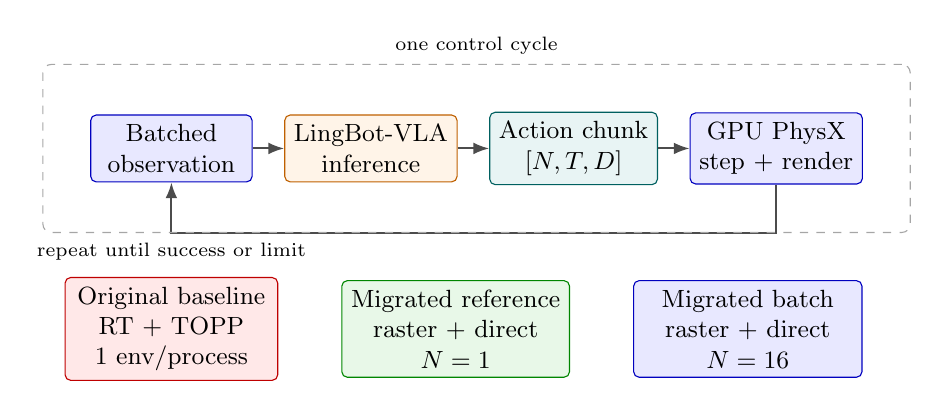
\begin{tikzpicture}[
  node distance=5mm and 4mm,
  block/.style={draw=#1!75!black, fill=#1!9, rounded corners=2pt, minimum width=2.05cm, minimum height=0.85cm, align=center, font=\small},
  arr/.style={-{Latex[length=2mm]}, line width=0.7pt, draw=black!70}
]
\node[block=blue] (obs) {Batched\\observation};
\node[block=orange, right=of obs] (vla) {LingBot-VLA\\inference};
\node[block=teal, right=of vla] (act) {Action chunk\\$[N,T,D]$};
\node[block=blue, right=of act] (phys) {GPU PhysX\\step + render};
\draw[arr] (obs) -- (vla);
\draw[arr] (vla) -- (act);
\draw[arr] (act) -- (phys);
\draw[arr] (phys.south) |- ++(0,-0.62) -| node[pos=.5,below,font=\scriptsize] {repeat until success or limit} (obs.south);
\node[draw=black!35, dashed, rounded corners=3pt, fit=(obs)(vla)(act)(phys), inner sep=6mm, label={[font=\scriptsize]above:one control cycle}] {};
\node[block=red, below=12mm of obs, minimum width=2.7cm] (base) {Original baseline\\RT + TOPP\\$1$ env/process};
\node[block=green!70!black, right=8mm of base, minimum width=2.7cm] (single) {Migrated reference\\raster + direct\\$N=1$};
\node[block=blue, right=8mm of single, minimum width=2.9cm] (batch) {Migrated batch\\raster + direct\\$N=16$};
\end{tikzpicture}
\caption{GPU 批量评测的闭环结构及三类执行配置。图中展示观测、模型推理、动作写入与物理推进的循环；原始基线使用 TOPP/RT，具体对照实验设置见表~\ref{tab:protocol}。}
\label{fig:pipeline}
\end{figure}

\subsection{实验设置}
实验使用 LingBot-VLA-v2 6B 的 \texttt{global\_step\_50000} 权重。全任务结果覆盖 RoboTwin 的 50 个任务：表~\ref{tab:protocol} 中的历史原始 TOPP/RT 基线每任务 100 集，共 5,000 集，其余配置每任务 16 集，共 800 集；迁移 N=16 的 randomized 评测同样为 800 集。后续代表任务对照另按各表注明的集数执行。成功率为成功集数除以评测集数。迁移管线采用 raster 渲染、direct 控制，每控制步最多 17 个物理子步，初始化稳定阶段为 2,500 个物理步。

原始 LingBot 单环境 TOPP/RT 作为基线，GPU 批量物理、批量动作与推理、direct 控制、raster 渲染及评测脚本适配共同构成迁移方案。整体系统比较保留这些必要改动；控制或渲染的独立贡献需要额外的单变量实验。历史全任务 GPU N=1 评测在同一仿真 GPU 上使用最多 3 个单环境 worker，N=16 则由单进程管理 16 个环境。后文小规模系统对照中的原始单环境方案均使用一个 slot，即同时只运行一个评测进程；批量方案也仅同时运行一个评测进程，进程内环境数为 N。

近期的小规模系统对照与规模实验复用对应任务的 seed 和已保存指令；历史全任务对照的匹配范围在各项结果中说明。规模实验进一步固定同一任务、seed 和动作块的采样噪声实现，但保留随机采样机制，不保证输出动作逐位一致。相同 seed 是场景生成的共同输入，也不等于已证明不同执行路径的初态逐位相同。

吞吐按评测集数除以已记录运行时间计算，并换算为集/小时。近期系统对照采用评测进程从启动至退出的耗时，多批次时求和，均不含 seed 筛选；全任务历史记录沿用其任务计时边界。进程耗时合计不包含完整调度等待和全部中断重跑，不能直接称为完整工作负载的总墙钟。历史 12 集实验的另一种计时边界见附录 A。

\begin{table}[htbp]
\centering\small
\caption{Clean 基线及对照实验。原始 TOPP/RT 基线为每任务 100 集，其余各组为每任务 16 集；各组均覆盖 50 个任务。}
\label{tab:protocol}
\begin{tabularx}{\textwidth}{@{}lYYcc@{}}
\toprule
评测管线 & 物理后端 / 环境数 & 控制 / 渲染 & 成功集数 & 成功率 \\
\midrule
原始基线 & 单环境 & TOPP / RT & 4486/5000 & 89.72\% \\
原始控制对照 & 单环境 & direct / RT & 732/800 & 91.50\% \\
单环境复刻评测 & CPU 单环境 & direct / raster & 662/800 & 82.75\% \\
迁移单环境 & CPU PhysX / N=1 & direct / raster & 681/800 & 85.13\% \\
迁移单环境 & GPU PhysX / N=1 & direct / raster & 657/800 & 82.13\% \\
早期迁移批量 & GPU PhysX / N=16 & direct / raster & 433/800 & 54.13\% \\
修复后迁移批量 & GPU PhysX / N=16 & direct / raster & 657/800 & 82.13\% \\
\bottomrule
\end{tabularx}
\end{table}

\subsection{Clean 全任务成功率：不同系统配置}
图~\ref{fig:success}(a) 比较各系统配置的总体成功率；原始 TOPP/RT 为 5,000 集，其余各组为 800 集。图~\ref{fig:success}(b) 对相同任务和 seed 的 800 集逐一比较 GPU N=1 与 N=16：两组均成功 615 集、仅 N=1 成功 42 集、仅 N=16 成功 42 集、两组均失败 101 集。因此两组总成功数同为 657，但有 84 集的成败不同。

\begin{figure}[htbp]
\centering
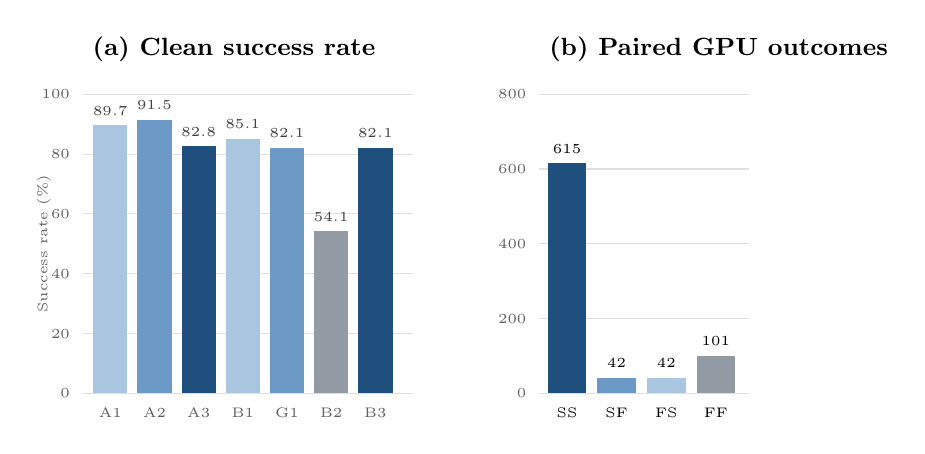
\begin{tikzpicture}[font=\scriptsize]
\begin{scope}[x=0.66cm,y=0.038cm]
\node[anchor=west,font=\small\bfseries] at (0,115) {(a) Clean success rate};
\foreach \y in {0,20,40,60,80,100} {\draw[gray!25] (0,\y) -- (6.35,\y); \node[anchor=east,text=gray!75!black,font=\tiny] at (-0.06,\y) {\y};}
\node[rotate=90,font=\tiny,text=gray!75!black] at (-0.75,50) {Success rate (\%)};
\foreach \x/\v/\c/\lbl in {0/89.72/chartLight/A1,0.85/91.5/chartMid/A2,1.7/82.75/chartDark/A3,2.55/85.125/chartLight/B1,3.4/82.125/chartMid/G1,4.25/54.125/chartGray/B2,5.1/82.125/chartDark/B3} {
\fill[\c] (\x+0.2,0) rectangle (\x+0.86,\v);
\node[above,font=\tiny,text=black!75] at (\x+0.53,\v) {\pgfmathprintnumber[fixed,precision=1]{\v}};
\node[below,font=\tiny,text=gray!75!black] at (\x+0.53,-1.5) {\lbl};}
\end{scope}
\begin{scope}[xshift=5.8cm,x=0.7cm,y=0.038cm]
\node[anchor=west,font=\small\bfseries] at (0,115) {(b) Paired GPU outcomes};
\foreach \y in {0,200,400,600,800} {\pgfmathsetmacro{\yy}{\y/8} \draw[gray!25] (0,\yy) -- (3.8,\yy); \node[anchor=east,text=gray!75!black,font=\tiny] at (-0.06,\yy) {\y};}
\fill[chartDark] (0.15,0) rectangle (0.85,76.875); \node[above,font=\tiny] at (0.5,76.875) {615};
\fill[chartMid] (1.05,0) rectangle (1.75,5.25); \node[above,font=\tiny] at (1.4,5.25) {42};
\fill[chartLight] (1.95,0) rectangle (2.65,5.25); \node[above,font=\tiny] at (2.3,5.25) {42};
\fill[chartGray] (2.85,0) rectangle (3.55,12.625); \node[above,font=\tiny] at (3.2,12.625) {101};
\node[below,font=\tiny] at (0.5,-1.5) {SS}; \node[below,font=\tiny] at (1.4,-1.5) {SF};
\node[below,font=\tiny] at (2.3,-1.5) {FS}; \node[below,font=\tiny] at (3.2,-1.5) {FF};
\end{scope}
\end{tikzpicture}
\caption{Clean 成功率与 GPU 单环境、批量评测的配对结果。(a) A1：原始 TOPP/RT 基线；A2：原始 direct/RT；A3：单环境复刻 direct/raster；B1：迁移 CPU N=1；G1：迁移 GPU N=1；B2、B3：修复前、后的 GPU N=16。A1 为 5,000 集，其余各组为 800 集。(b) 对同一任务和 seed，依次记录 GPU N=1、N=16 的成功（S）或失败（F）：SS 为两组均成功，SF 为仅 N=1 成功，FS 为仅 N=16 成功，FF 为两组均失败。}
\label{fig:success}
\end{figure}
\textbf{控制方式。}原始 LingBot 单环境使用 TOPP 和 RT 的基线成功率为 4486/5000（89.72\%）；关闭 TOPP、采用 direct 控制并保持 RT 后为 732/800（91.50\%），相差 1.78 个百分点。两组分别为每任务 100 集和 16 集，运行并发及策略随机流也不完全相同；现有结果可用于观察控制配置变化下的总体表现，尚不能判断 direct 的成功率必然更高。

\textbf{渲染配置与系统表现。}原始单环境 direct/RT 取得 732/800（91.50\%），采用 raster 的单环境复刻方案取得 662/800（82.75\%），后者低 8.75 个百分点。这两组均执行 50 个任务、每任务 16 集，展示了两套单环境配置的实际结果。第二组的评测脚本是系统适配的一部分；该差值反映包含渲染与执行路径在内的整体配置变化，可用于评估采用 raster 方案后的系统表现。若需要量化渲染组件单独贡献，再补充固定其余条件的实验。

\textbf{迁移路径与物理后端。}两次 direct/raster CPU 单环境方案分别为 662/800（82.75\%）和 681/800（85.13\%），后者高约 2.38 个百分点；两组为不同运行，具体代码版本与适配差异仍需溯源。迁移 CPU N=1 与 GPU N=1 方案分别为 681/800（85.13\%）和 657/800（82.13\%），GPU 方案低 3.00 个百分点；两组使用相同任务和 seed 清单，800 集中有 100 集的成败不同。物理后端和相应执行路径属于各自方案，这些结果描述系统方案的总体与逐集差异。

\textbf{批量规模。}GPU N=1 与 N=16 的总体结果均为 657/800（82.13\%），但 800 个任务--seed 配对中有 84 个成败不同，涉及 33 个任务；仅 N=1 成功和仅 N=16 成功各 42 集。批量推理是 N=16 方案的组成部分，故该结果是两套完整方案的成功率比较。N=1 最多三个单环境 worker，N=16 为一个批量进程；逐 seed 分歧用于展示不同样本的结果，不影响报告两组总体成功数一致。表~\ref{tab:tasks} 给出代表任务的结果。

\textbf{共享管线修复。}早期批量运行按旧统计口径记录 433/800，修复后记录 657/800，增加 224 集，即 28.00 个百分点；早期未锁存成功状态，可能漏记曾经成功的环境。修复包含 GPU 状态初始化与写入、共享碰撞地面和成功状态锁存；早期运行还使用不同求解器设置，因此该变化反映综合系统修正，不是某一项修改的独立效果。

\begin{table}[htbp]
\centering\small
\caption{代表任务的 clean 成功集数及 GPU 配对结果差异，每组各 16 集。}
\label{tab:tasks}
\begin{tabular}{@{}lcccc@{}}
\toprule
任务 & CPU N=1 & GPU N=1 & GPU N=16 & GPU 配对分歧 \\
\midrule
\texttt{beat\_block\_hammer} & 15 & 8 & 9 & 5 \\
\texttt{open\_microwave} & 13 & 13 & 12 & 3 \\
\texttt{stack\_blocks\_three} & 10 & 9 & 9 & 6 \\
\texttt{place\_fan} & 16 & 10 & 8 & 8 \\
\bottomrule
\end{tabular}
\end{table}

\subsection{Clean 逐任务表现}
总体成功率能够概括全部任务，但会掩盖各任务之间的差异。图~\ref{fig:taskprofiles} 将 CPU N=1、GPU N=1 和 GPU N=16 的每任务成功率放在相同任务顺序下比较：在同一任务位置比较三个点，可以看出各方案在该任务上的表现差异；连线仅帮助辨认各方案，不表示任务随横轴连续变化。三组均采用 direct/raster，每任务 16 集，并使用相同任务和 seed 清单。GPU N=1 与 N=16 的总体成功数均为 657，但 50 个任务中有 29 个任务的成功数不同；其中 33 个任务存在至少一集的逐 seed 成败差异。批量推理、GPU 环境管理与相应评测适配是各方案的组成部分，图中结果用于比较各方案的完整任务表现。

代表任务中，\texttt{place\_fan} 的 CPU N=1、GPU N=1 和 GPU N=16 分别为 16/16、10/16 和 8/16；\texttt{stack\_blocks\_three} 分别为 10/16、9/16 和 9/16，后两组总数相同但有 6 个 seed 的结果不同。这些任务级结果为后续选择针对性诊断提供依据，不单独代表整体表现。

\begin{figure}[htbp]
\centering
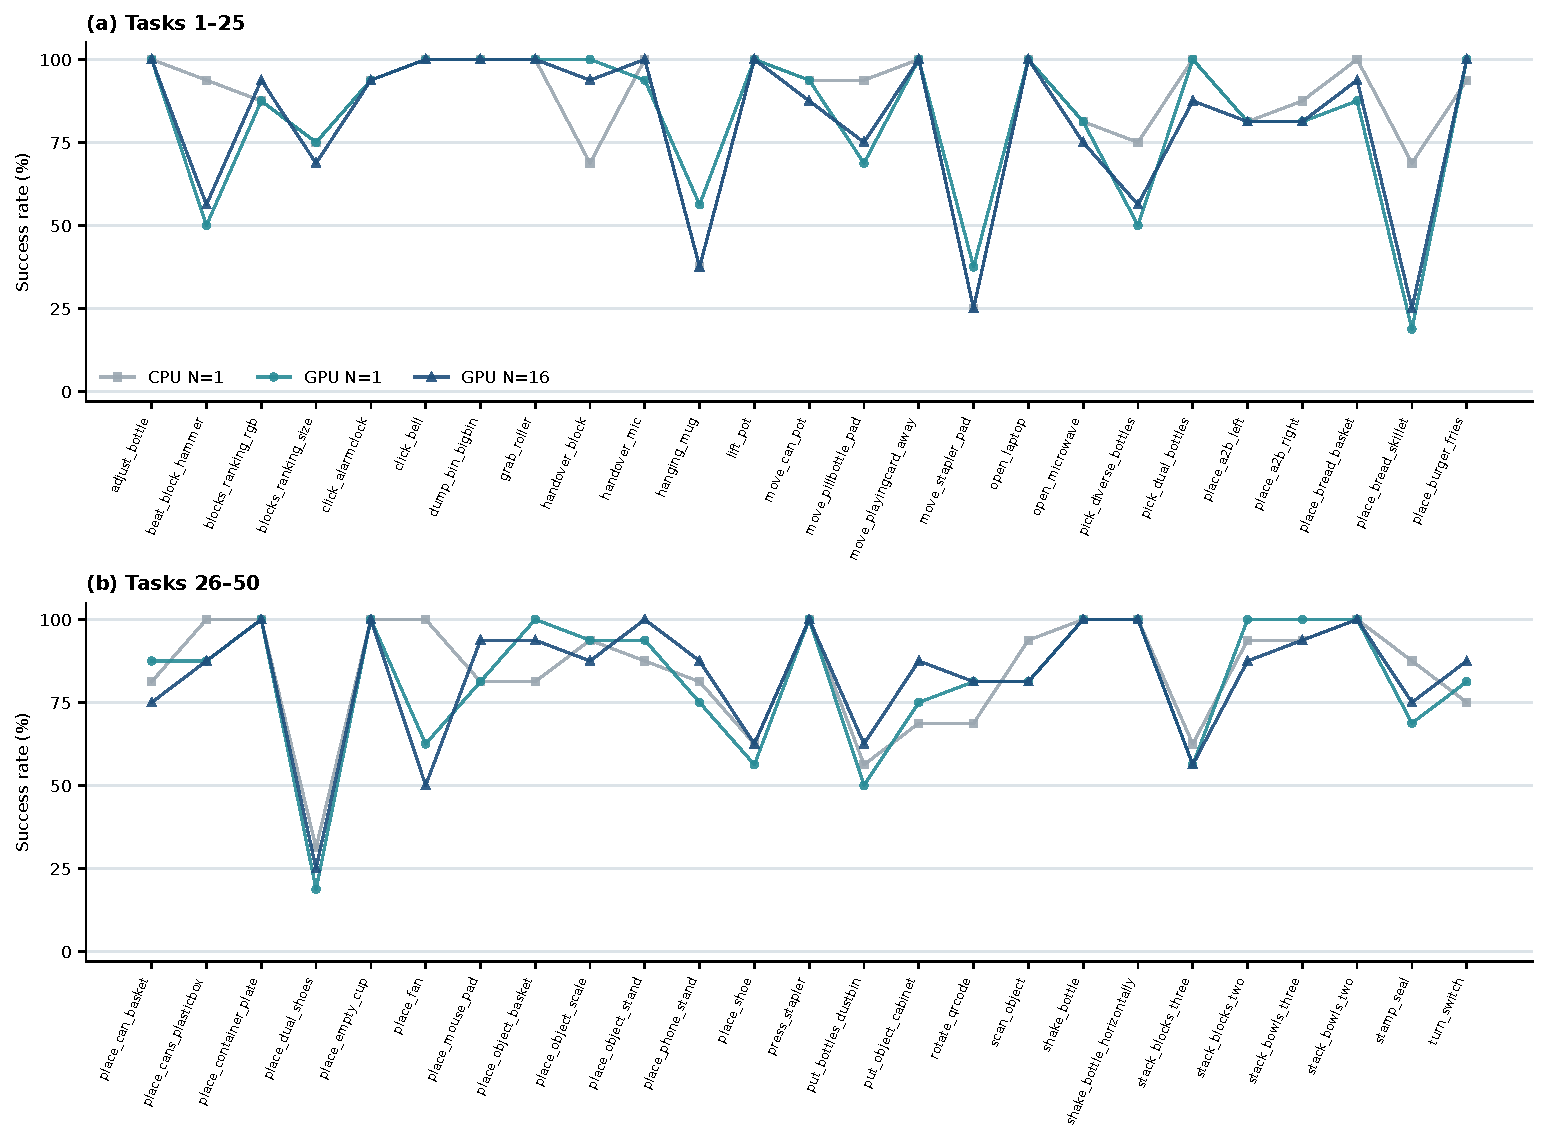
\includegraphics[width=\textwidth]{figures/clean_task_profiles.pdf}
\caption{Clean 逐任务成功率。(a)、(b) 分别展示按任务名称排序的前 25 个和后 25 个任务；每个点由对应方案的 16 集计算。CPU N=1、GPU N=1、GPU N=16 使用相同任务与 seed 清单，direct 控制和 raster 渲染。连线用于辨认各离散任务的方案结果，不表示任务之间的连续变化；每任务 1 集对应 6.25 个百分点。}
\label{fig:taskprofiles}
\end{figure}

\subsection{Clean 与 randomized 全任务表现}
Randomized 配置改变背景纹理、桌面杂物、光照及桌面高度，评测模式使用 unseen 背景纹理。表~\ref{tab:cleanrandom} 对照迁移 GPU N=16 在两种场景下的 50 任务结果。Randomized 成功 648/800（81.00\%），比 clean 的 657/800（82.13\%）低约 1.13 个百分点。两种场景各自使用通过专家检查的 seed，因而该差值描述各场景评测样本上的总体表现，不能单独解释为随机化因素的因果影响。原始 TOPP/RT 在同一组 randomized 样本上的全任务结果仍待补充。

\begin{table}[htbp]
\centering\small
\caption{迁移 GPU N=16 的 clean 与 randomized 全任务评测，各 50 个任务、每任务 16 集。进程耗时为任务耗时之和，不含专家筛选和全部中断、重跑，不是连续完整墙钟。}
\label{tab:cleanrandom}
\begin{tabular}{@{}lrrr@{}}
\toprule
场景 & 成功率 & 进程耗时（秒） & 吞吐（集/小时） \\
\midrule
Clean & 657/800（82.13\%） & 14851.97 & 193.9 \\
Randomized & 648/800（81.00\%） & 17360.90 & 165.9 \\
\bottomrule
\end{tabular}
\end{table}

\subsection{逐项修复的任务级验证}
表~\ref{tab:repair} 汇总已记录的修复前后结果。固定动作回放重复执行相同 VLA 动作，用于观察物理执行或统计的变化；真实闭环在运行中根据观测重新生成动作。两者回答的问题不同，结果分别标记。

\begin{table}[htbp]
\centering\small
\caption{代表性共享管线修复的任务级结果，每组 N=16。固定动作回放与真实 VLA 闭环分别列出。}
\label{tab:repair}
\begin{tabularx}{\textwidth}{@{}l l c c Y@{}}
\toprule
修复 & 任务 & 前 & 后 & 验证方式与范围 \\
\midrule
成功锁存 & 堆叠两个积木 & 9/16 & 15/16 & 固定动作；修正成功状态漏记 \\
成功锁存 & 锤击 & 13/16 & 16/16 & 单地面，同 seed 固定动作 \\
共享地面 & 锤击 & 11/16 & 15/16 & 固定动作；单个样本组 \\
关节初值 & 打开笔记本 & 14/16 & 16/16 & 真实 VLA 闭环，同 seed \\
根位姿初始化 & 锤击 & 12/16 & 11/16 & 固定动作；本组成功数未改善 \\
\bottomrule
\end{tabularx}
\end{table}

上述锁存回放反映成功统计方式的修正；共享地面回放显示该动作组的执行结果变化。笔记本的闭环前后成功数来自不同运行，原始记录中模型采样未完全固定。逐项真实闭环前后数据尚未覆盖全部修复与任务，后续根据需要补测。

\subsection{Clean 与 randomized 小规模系统对照}
为比较完整系统的运行效率，在 clean 和 randomized 场景下分别选取 \texttt{click\_bell}、\texttt{beat\_block\_hammer} 和 \texttt{pick\_diverse\_bottles}。每个任务评测 16 集，各场景下两套系统使用相同的 seed 和指令；原始 TOPP/RT 使用单 slot，迁移方案使用单进程 N=16 direct/raster。表~\ref{tab:smallcompare} 的耗时为三个任务的评测进程耗时合计，不包含 seed 筛选、完整调度等待及全部中断重跑。

\begin{table}[htbp]
\centering\small
\caption{三任务小规模系统对照。每个场景、每套系统均评测 48 集，吞吐按任务进程耗时合计计算。}
\label{tab:smallcompare}
\begin{tabular}{@{}llrrr@{}}
\toprule
场景 & 系统 & 成功率 & 耗时（秒） & 吞吐（集/小时） \\
\midrule
Clean & 原始 TOPP/RT & 41/48（85.42\%） & 1425.01 & 121.3 \\
 & 迁移 N=16 & 37/48（77.08\%） & 748.01 & 231.0 \\
\midrule
Randomized & 原始 TOPP/RT & 36/48（75.00\%） & 1981.93 & 87.2 \\
 & 迁移 N=16 & 37/48（77.08\%） & 788.94 & 219.0 \\
\bottomrule
\end{tabular}
\end{table}

图~\ref{fig:smallcompare} 对照两套系统的成功率和吞吐。迁移方案的记录吞吐在 clean 和 randomized 下分别为原始方案的约 1.91 倍和 2.51 倍；成功数分别少 4 集和多 1 集。该结果描述本次三个任务的完整系统配置，不代表单一组件的贡献或 50 任务整体加速比，后续将补充全任务对照。

\begin{figure}[htbp]
\centering
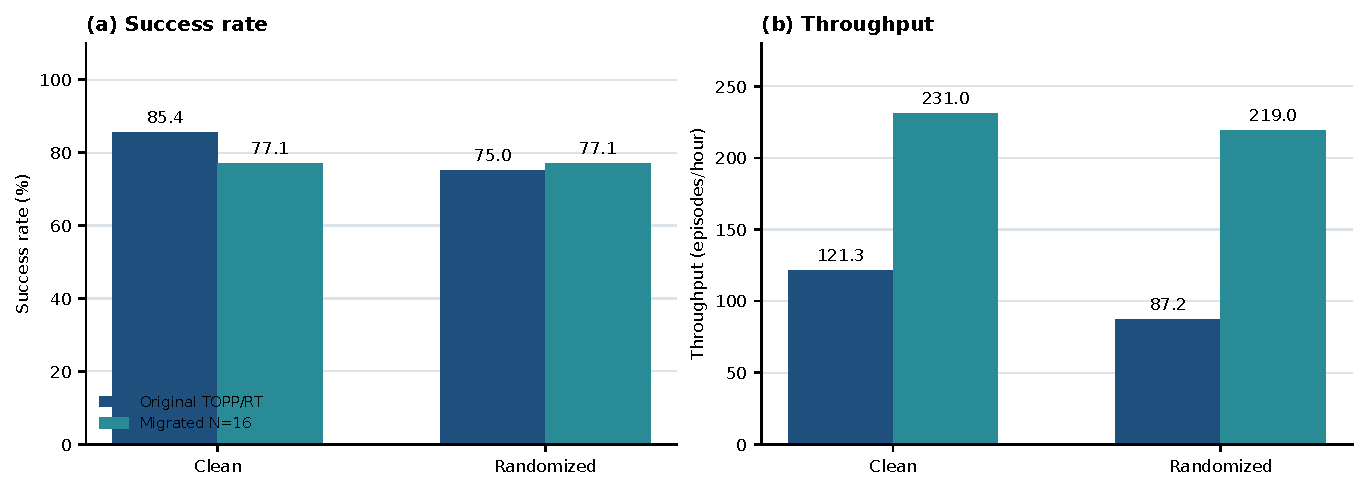
\includegraphics[width=\textwidth]{figures/small_system_compare.pdf}
\caption{Clean 和 randomized 下的三任务系统对照。(a) 为成功率，(b) 为按任务进程耗时合计计算的吞吐；每个场景、每套系统共 48 集，同场景两套系统使用相同 seed 和指令。}
\label{fig:smallcompare}
\end{figure}

\subsection{两任务系统吞吐与成功率对照}
为观察不同任务是否有相似的系统收益，原始单环境 TOPP/RT 与迁移 N=16 direct/raster 分别评测 \texttt{click\_bell} 和 \texttt{beat\_block\_hammer}，每任务使用相同的 64 个 clean seed 和指令。原始方案采用单 slot；迁移方案以 4 个 N=16 批次依次执行，数据取自后文表~\ref{tab:three128} 的前四批，不是另一组独立重复。进程耗时从评测进程启动计至退出，不包含专家筛选。迁移侧采用逐环境采样噪声控制，原始侧使用原服务的采样流，结果按各自完整方案报告。

\begin{table}[htbp]
\centering\small
\caption{两个 clean 任务的系统对照，每组 64 集。迁移方案采用 4 个 N=16 批次，进程耗时按批次累加；吞吐不含 seed 筛选。当前仅覆盖两个任务，完整 50 任务对照后续补充。}
\label{tab:twotask}
\begin{tabular}{@{}llrrrr@{}}
\toprule
任务 & 系统 & 成功率 & 耗时（秒） & 吞吐（集/小时） & 相对吞吐 \\
\midrule
\texttt{click\_bell} & 原始 TOPP/RT & 35/64（54.69\%） & 2302.38 & 100.1 & 1.00$\times$ \\
 & 迁移 N=16 & 62/64（96.88\%） & 466.98 & 493.4 & 4.93$\times$ \\
\midrule
\texttt{beat\_block\_hammer} & 原始 TOPP/RT & 58/64（90.63\%） & 1804.88 & 127.7 & 1.00$\times$ \\
 & 迁移 N=16 & 44/64（68.75\%） & 781.10 & 295.0 & 2.31$\times$ \\
\bottomrule
\end{tabular}
\end{table}

图~\ref{fig:twotask} 将表~\ref{tab:twotask} 的成功率与吞吐画在一起：每条线对应一个任务，左、右两点分别为原始和迁移方案。两个任务的迁移系统吞吐均高于对应原始方案；敲铃的迁移成功数更高，锤击则低于原始方案。成功率和各集实际执行步数的变化也会影响耗时，因此这些倍数描述本次完整系统运行，不代表单一组件的收益或 50 任务的整体加速比。

\begin{figure}[htbp]
\centering
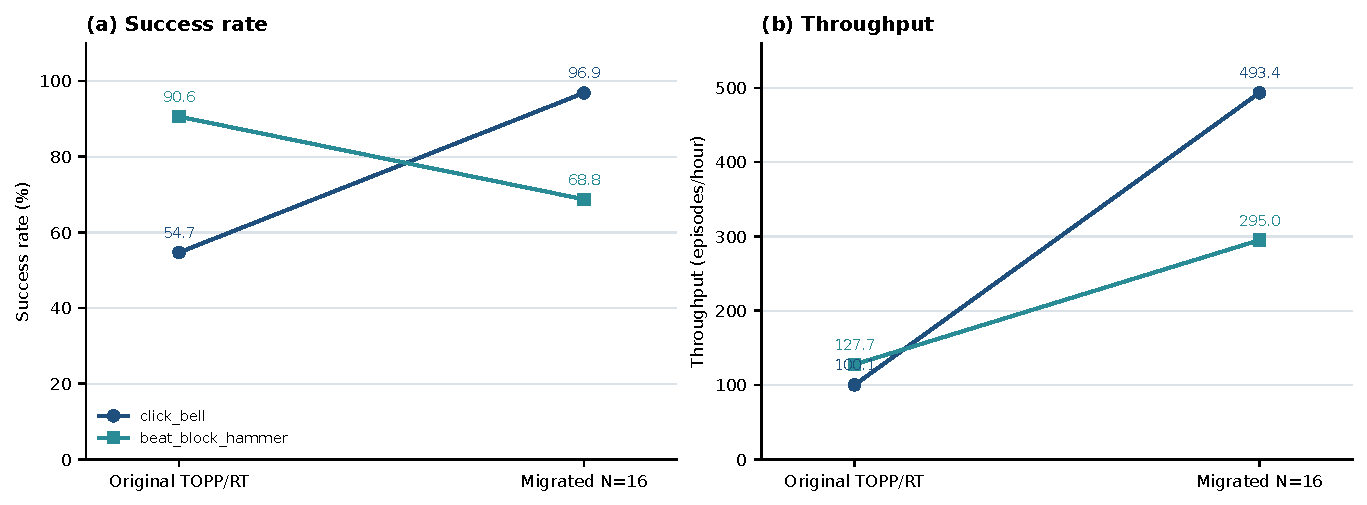
\includegraphics[width=\textwidth]{figures/clean_two_task_systems.pdf}
\caption{两个 clean 任务的系统成功率与吞吐。每组使用相同的 64 个 seed 和指令；(a) 比较成功率，(b) 比较吞吐。每条线连接同一任务的原始与迁移方案，仅表示两次系统结果。当前仅覆盖两个任务，后续补充完整任务对照。}
\label{fig:twotask}
\end{figure}

\subsection{锤击任务的固定动作诊断}
为区分 VLA 生成动作与物理执行的影响，锤击任务在相同 64 个 seed 和指令下进行两次 N=64 闭环；保存第一次闭环的动作并在 N=64 下回放。表~\ref{tab:hammerreplay} 将真实闭环和固定动作回放分开报告。

\begin{table}[htbp]
\centering\small
\caption{锤击任务的真实闭环与固定动作回放，每组 64 集。}
\label{tab:hammerreplay}
\begin{tabular}{@{}llr@{}}
\toprule
运行方式 & 环境数 & 成功率 \\
\midrule
真实 VLA 闭环，第 1 次 & N=64 & 48/64（75.00\%） \\
真实 VLA 闭环，第 2 次 & N=64 & 38/64（59.38\%） \\
回放第 1 次的动作 & N=64 & 48/64（75.00\%） \\
\bottomrule
\end{tabular}
\end{table}

N=64 固定动作回放与第一次闭环的逐 seed 成败结果一致，表明本次回放能够重现原闭环结果，未观察到明显的物理执行异常；这一结果仅覆盖锤击任务及该组动作，物理执行的整体表现仍需更多任务和全量评测验证。两次真实 VLA 闭环的成功数分别为 48/64 和 38/64，存在运行间差异；当前实验尚不能确定差异来源，后续通过控制采样及初态并增加重复实验分析。

此外，历史 CPU/GPU 固定动作回放中，锤击、微波炉和放置风扇任务均存在 CPU 单环境成功而 GPU N=1 失败的样本；资产检查也发现两条路径的碰撞凸包和惯量读数存在差异。这些跨后端观察与上述同一 GPU 路径的 N=64 回放回答不同问题：前者提示两套系统的执行差异，后者检验本组动作能否重现。因此，同路径回放一致不能排除全部 CPU/GPU 差异，也不足以将闭环波动归因于某一种物理机制。

\subsection{单进程环境规模扩展}
\subsubsection{N=16 参考配置}
为考察扩大环境数的收益与代价，在 clean 场景下选择敲铃、锤击和多物体抓取三个任务，分别涉及接触触发、工具操作与多物体场景；它们不代表全部 50 个任务。每任务先使用 128 个通过专家检查的 seed，分 8 批依次启动 N=16 评测进程，建立规模对照的参考结果。表~\ref{tab:three128} 给出成功率与按进程耗时合计计算的吞吐。每任务复用历史原始评测中已通过专家检查的 100 个 seed，并补充筛选 28 个；筛选耗时不计入表中。策略请求按任务、环境 seed 和动作块序号生成独立采样噪声，重复编号固定为 0，并记录噪声标识。

\begin{table}[htbp]
\centering\small
\caption{Clean 三任务的 N=16 扩展评测，每任务 128 集。进程耗时为八个批次的耗时合计，不包含 seed 筛选。}
\label{tab:three128}
\begin{tabular}{@{}lrrr@{}}
\toprule
任务 & 成功率 & 进程耗时（秒） & 吞吐（集/小时） \\
\midrule
\texttt{click\_bell} & 122/128（95.31\%） & 1138.99 & 404.6 \\
\texttt{beat\_block\_hammer} & 90/128（70.31\%） & 1561.87 & 295.0 \\
\texttt{pick\_diverse\_bottles} & 78/128（60.94\%） & 1650.11 & 279.3 \\
\bottomrule
\end{tabular}
\end{table}

\subsubsection{扩展至 N=200}
在表~\ref{tab:three128} 的基础上，对相同三个 clean 任务分别测试 N=32、64、128 和 200。N=16、32、64 和 128 各使用相同的 128 个 seed 和指令，分别依次执行 8、4、2 和 1 批。N=200 复用上述 128 个 seed 和指令，再补充 72 个通过专家检查的 seed，以单批评测 200 集。各规模按任务、环境 seed 和动作块序号生成相同的逐环境随机采样噪声；N=200 的前 128 集与此前使用相同指令，已逐项核验。表~\ref{tab:scaling} 的进程耗时为各批次耗时之和，吞吐以实际评测集数除以该耗时计算，不含 seed 筛选及完整调度耗时。

\begin{table}[htbp]
\centering\small
\caption{三个 clean 任务在不同单进程环境数下的结果。N=16 至 128 每组 128 集，N=200 每组 200 集；成功率按各组全部样本计算。耗时为任务评测进程耗时之和，不含 seed 筛选。}
\label{tab:scaling}
\begin{tabular}{@{}lrrrr@{}}
\toprule
任务 & $N$ & 成功率 & 耗时（秒） & 吞吐（集/小时） \\
\midrule
\texttt{click\_bell} & 16 & 122/128（95.31\%） & 1138.99 & 404.6 \\
 & 32 & 122/128（95.31\%） & 1259.48 & 365.9 \\
 & 64 & 122/128（95.31\%） & 919.91 & 500.9 \\
 & 128 & 123/128（96.09\%） & 796.91 & 578.2 \\
 & 200 & 194/200（97.00\%） & 1175.81 & 612.3 \\
\midrule
\texttt{beat\_block\_hammer} & 16 & 90/128（70.31\%） & 1561.87 & 295.0 \\
 & 32 & 94/128（73.44\%） & 1128.57 & 408.3 \\
 & 64 & 92/128（71.88\%） & 897.54 & 513.4 \\
 & 128 & 93/128（72.66\%） & 767.78 & 600.2 \\
 & 200 & 149/200（74.50\%） & 1201.08 & 599.5 \\
\midrule
\texttt{pick\_diverse\_bottles} & 16 & 78/128（60.94\%） & 1650.11 & 279.3 \\
 & 32 & 75/128（58.59\%） & 1183.67 & 389.3 \\
 & 64 & 77/128（60.16\%） & 914.48 & 503.9 \\
 & 128 & 81/128（63.28\%） & 783.46 & 588.2 \\
 & 200 & 122/200（61.00\%） & 1169.22 & 615.8 \\
\bottomrule
\end{tabular}
\end{table}

图~\ref{fig:scaling}(a) 在各规模共同的 128 个 seed 上比较成功率。N=128 与 N=200 的敲铃成功数分别为 123 和 122，锤击为 93 和 97，瓶子抓取为 81 和 77。本轮三个任务未观察到成功率随环境数增加而持续下降的共同趋势，尚无证据将个别波动归因于资源竞争。总体成功数接近也不意味着逐集一致：锤击在 N=16 与 N=128 下有 45 个 seed 的成败不同。固定采样噪声不保证模型输出逐位一致，仍需独立重复分析波动。

图~\ref{fig:scaling}(b) 显示大规模下的吞吐收益趋缓。N=128 增至 N=200 后，敲铃和瓶子抓取的记录吞吐分别提高约 5.9\% 和 4.7\%，锤击基本持平。三个任务在 N=200 时分别耗时 1175.81、1201.08 和 1169.22 秒，均高于各自 N=128 的记录；但评测量也由 128 集增至 200 集，增加了 56.25\%，不能将总耗时增加直接解释为处理同等工作量更慢。图~\ref{fig:scaling}(d) 因此报告进程耗时除以集数：N=128 至 N=200，敲铃由约 6.23 降至 5.88 秒/集，锤击由 6.00 变为 6.01 秒/集，瓶子抓取由 6.12 降至 5.85 秒/集。这些是批量运行的平均处理成本，不是单集独立执行的延迟。

\begin{figure}[htbp]
\centering
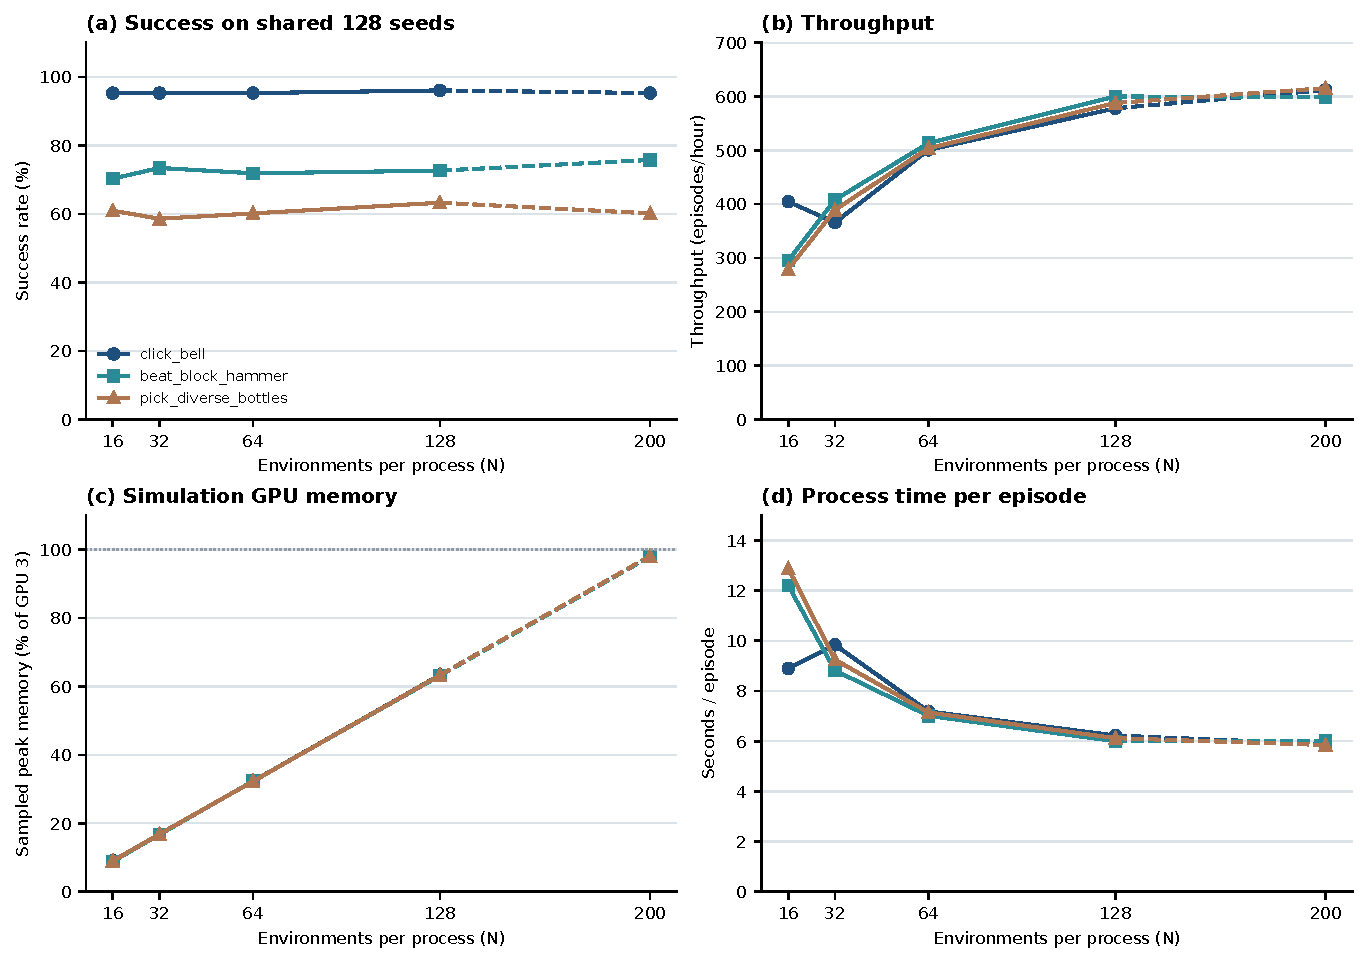
\includegraphics[width=\textwidth]{figures/clean_scaling.pdf}
\caption{三个 clean 任务的环境规模对照，每条线对应一个任务。(a) 为各规模共同 128 个 seed 的成功率；(b) 为实际评测集数除以进程耗时合计所得的吞吐；(c) 为仿真卡显存采样峰值占比，水平点线标记单卡容量，三个任务的曲线近乎重合；(d) 为进程耗时除以集数。N=16 至 128 各评测 128 集，N=200 评测 200 集；连接至 N=200 的线段用虚线标记这一工作量变化。横轴按实际环境数取值。}
\label{fig:scaling}
\end{figure}

图~\ref{fig:scaling}(c) 显示，仿真卡为总显存 143,771 MiB 的 H200 NVL，N=128 时三个任务的显存采样峰值约为单卡的 63.1\%--63.3\%，N=200 时升至 98.0\%--98.1\%。本轮 N=200 均完成评测，但显存余量已很小，因而可视为当前硬件、任务和配置下接近显存容量的工作点，尚不能认定为所有任务的环境数上限。结合吞吐结果，本轮观察到继续扩大环境数的效率收益已明显减小；是否为稳定的吞吐饱和区间，以及具体瓶颈所在，仍需阶段计时和重复实验确认。

规模实验使用 GPU 2 执行策略推理、GPU 3 执行仿真；部分运行期间其他实验共享主机 CPU、内存和 I/O，各组负载不完全相同。服务预热、实际执行步数和 N=200 新增样本也可能影响耗时。因此上述结果仅描述三个 clean 任务的本轮运行，还需补充固定总工作量的独立重复、更多任务与 randomized 场景。

\subsection{现有对照的解释范围}
表~\ref{tab:dimensions} 将现有数据按比较维度归纳。当前结果可用于描述各次运行的总体与逐任务表现。系统级比较保留各方案的必要改动；如需拆分控制、渲染或物理后端的独立作用，再单独对照。

\begin{table}[htbp]
\centering\small
\caption{现有比较及其证据边界。}
\label{tab:dimensions}
\begin{tabularx}{\textwidth}{@{}lYY@{}}
\toprule
维度 & 已有观察 & 比较范围 \\
\midrule
控制 & TOPP/RT 89.72\%；direct/RT 91.50\% & 集数、并发和随机流不同 \\
单环境渲染配置 & direct/RT 91.50\%；复刻 direct/raster 82.75\% & 整体配置差 8.75 个百分点 \\
物理与执行路径 & CPU N=1 85.13\%；GPU N=1 82.13\% & 两套系统差 3.00 个百分点 \\
批量规模 & 两套方案均 82.13\%，84 集成败不同 & N=1 至多三 worker，N=16 单进程；记录逐集结果 \\
系统修正 & 旧批量 54.13\%；修复后 82.13\% & 统计口径、求解器和多项代码修复 \\
场景变化 & Clean 82.13\%；randomized 81.00\% & 各 800 集，各自专家通过 seed；总体表现对照 \\
系统吞吐 & 三任务 clean/随机化为 1.91/2.51 倍；两任务分别为 4.93/2.31 倍 & 同场景两套系统使用相同 seed 和指令；按进程耗时计算，样本组不同 \\
规模与资源 & 三任务扩展至 N=200，显存峰值约 98\%；N=128 后吞吐收益趋缓 & 仅本轮 clean 任务；N=200 的评测量由 128 增至 200 集 \\
\bottomrule
\end{tabularx}
\end{table}

\section{真机部署}
% 后续补充机器人平台与部署实验。
\section{结论}
GPU 并行评测管线已完成 50 任务的 clean 与 randomized 评测，分别成功 657/800 和 648/800 集。Clean 的 GPU N=1 与 N=16 总成功数相同，但逐集结果存在差异。三任务小规模系统对照中，迁移方案在两个场景的记录吞吐均高于原始 TOPP/RT；两任务的扩展对照进一步显示，效率收益伴随不同方向的任务成功率变化，不能以吞吐提高推断成功率保持不变。三个 clean 任务均扩展至 N=200，在共同样本上未观察到成功率随规模持续下降的共同趋势；仿真卡显存采样峰值约为容量的 98\%，N=128 至 N=200 的吞吐收益趋缓。现有结果支持继续开展全任务系统效率验证，尚不足以确定全任务加速比、普遍环境数上限或单一组件的独立收益。

\section{实验补充计划}
后续实验以相同任务、seed、指令、模型和任务步数上限为基础，分别记录筛选、初始化、闭环、任务切换及完整墙钟。完整系统比较保留各方案的必要实现；记录服务精度、GPU 分配和并发，并对齐计时范围。分阶段计时应标明包含关系及 GPU 同步边界；若需相加解释总耗时，使用互不重叠的阶段，避免重复累计动作内部的物理与目标上传时间。

\textbf{完整系统吞吐。}在完成代表任务对照后，继续单环境 clean TOPP/RT、randomized TOPP/RT 和 randomized direct/raster，各组均为 50 任务、每任务 16 集，使用对应批量结果的固定 seed 与已保存指令，单环境采用一个 slot，不重复运行 expert；筛选时间单独记录，分别核对批量与单环境的进程计时及完整调度时间。调整后的单环境入口使用无动作的任务状态初始化，其与原始流程的状态一致性尚待核验。现有 clean N=16 的 14,852 秒为已完成任务时间之和，需按一致的计时范围核验或补测，才可用于严格的总墙钟比。

\textbf{控制与渲染。}在需要分析单项技术时，在同一单环境入口、相同渲染配置下比较 TOPP 与 direct；再在固定控制、模型和 seed 下比较 RT 与 raster。两组分别保存任务结果及耗时；随机流与实际指令需记录或固定。

\textbf{物理与批量规模。}已有锤击 N=64 同路径回放及三个任务 N=16 至 200 的单次规模结果。后续先在固定总工作量与资源条件下增加独立重复，沿用逐环境采样噪声规则，报告逐 seed 差异与不确定性；若出现稳定的任务成功率下降，再通过保存初态、观测与动作，补充针对性的 CPU/GPU 和跨 N 固定动作回放，区分策略与执行差异。

\textbf{并发、批量规模与瓶颈。}完成 clean 和 randomized 的基线对齐后，在固定 GPU 分配、任务、seed、指令、模型和计时范围下，扫描迁移系统的进程数 $M$ 与每进程环境数 $N$；同时运行 $M$ 个评测进程，每个进程管理 $N$ 个环境。各组合处理相同的总任务量，记录完整墙钟、吞吐、总体及逐任务成功率，以及 GPU 显存、利用率和策略服务负载。结合初始化、仿真、渲染与推理等阶段耗时，判断吞吐随 $M$、$N$ 增长何时趋于饱和及可能的瓶颈。以已对齐结果为参考，结合重复实验考察成功率变化，在满足约定的成功率要求后选择配置；可接受差异与具体扫描范围在正式测试前确定。原始单环境的 slot 数也可独立扫描，用于系统级资源对照。

\appendix
\section{实验记录与复现材料}
工作区保留 clean 评测的 seed 清单、逐任务结果以及 GPU N=1 与 N=16 的逐 seed 对照。总体结果见成功率多维对比报告，randomized 全量实验分别记录专家筛选结果与批量评测结果。这些本地材料对应当前版本，公开发布材料尚待整理。

\subsection{历史单任务吞吐记录}
早期 \texttt{pick\_diverse\_bottles} 单任务实验使用同一组 12 个 seed，最大控制步数为 400。单环境 TOPP/RT 以 12 个独立进程逐个串行执行，每集记录的初始化与闭环耗时之和累计为 693.3 秒；批量 direct/raster 以单进程 N=12 执行，记录的初始化加闭环耗时为 168.8 秒。两组成功数均为 7/12。按这两个计时值计算，吞吐分别为 62.3 和 255.9 集/小时，比值为 4.11。单环境计时合计不包含进程间启动等待，批量计时取初始化与闭环阶段之和，因此该比值是单任务、所记录阶段的系统配置对照，不是完整调度墙钟比。两组的控制、渲染、物理子步数和并发方式不同，该结果不能归因于单一技术，也不能外推为 50 个任务的加速比。

\clearpage
\section{迁移实现对照与后续优化（截至 2026 年 11 月 20 日）}
\label{app:implementation}
本节以 ManiSkill3 的 SAPIEN 3.0 路径为参照，归纳当前 RoboTwin 迁移的实现范围。已实现表示相应功能已接入评测闭环；核心机制沿用不表示任务、物理参数、控制器或性能完全相同。技术实现状态与实验验证范围分别判断，现有规模测试尚不足以确定各环节的独立收益。

\begingroup
\small
\setlength{\tabcolsep}{4pt}
\begin{longtable}{@{}>{\raggedright\arraybackslash}p{0.14\textwidth}>{\raggedright\arraybackslash}p{0.24\textwidth}>{\raggedright\arraybackslash}p{0.29\textwidth}>{\raggedright\arraybackslash}p{0.25\textwidth}@{}}
\caption{ManiSkill3 与当前迁移实现的对照。状态对应截至 2026 年 11 月 20 日的代码与已有实验；优化方向尚待阶段测量和成功率验证。}\label{tab:implementationaudit}\\
\toprule
环节与状态 & ManiSkill3 的做法 & 当前迁移实现 & 后续可参考的优化 \\
\midrule
\endfirsthead
\multicolumn{4}{l}{\tablename~\thetable\ （续）}\\
\toprule
环节与状态 & ManiSkill3 的做法 & 当前迁移实现 & 后续可参考的优化 \\
\midrule
\endhead
\midrule
\multicolumn{4}{r}{续下页}\\
\endfoot
\bottomrule
\endlastfoot
GPU 多环境物理\newline 已实现 & 共享 GPU 物理系统，批量推进多个环境。 & 一个 GPU PhysX 系统管理多个 RoboTwin 子场景，通过空间偏移组织环境；保留所需的 RoboTwin 物理配置。 & 分别测量各调用开销，继续探索环境数 $N$ 与进程数 $M$ 的资源和吞吐关系。 \\
\addlinespace
相机组批量渲染\newline 已实现 & 按相机视角组织相机组，获取多环境图像。 & 已采用同类 SAPIEN 相机组接口，不同组依次调用；组内后端逐相机发起渲染，输出批量 GPU 图像。 & 测量渲染、等待、图像读取与 GPU 执行时间线；批量接口不保证所有画面严格同时执行。 \\
\addlinespace
GPU 图像获取\newline 已实现 & 从 CUDA 图像缓冲获取 Torch 张量。 & 同样取得批量 CUDA 图像张量；该环节的核心接口已经接入。 & 在已有 GPU 图像基础上优化预处理及其后续传输。 \\
\addlinespace
观测传给模型\newline 部分实现 & 提供 GPU 张量观测；直接集成的策略可消费这些张量，具体模型部署由使用者决定。 & 图像读回 CPU 并转为 NumPy，再经 WebSocket 请求独立 VLA 服务；未形成端到端 GPU 数据链路。 & 研究 GPU 图像预处理、同进程模型调用，或保留服务并增加 GPU 数据共享和跨卡传输。 \\
\addlinespace
批量 VLA 推理\newline 已完成适配 & 框架支持批量环境交互，不统一规定 VLA 的部署和服务方式。 & LingBot-VLA 服务接收批量观测、返回各环境动作块；保留 WebSocket 服务机制，仿真与模型分别使用 GPU。 & 分开测量通信、预处理和模型计算，再决定服务与数据接口的优化。 \\
\addlinespace
动作与控制\newline 已实现并适配 & 批量控制器支持关节位置、增量及末端控制等配置，物理子步数随设置变化。 & 相对原始 RoboTwin 关闭 TOPP，采用 direct、每控制动作最多 17 个物理子步；批量写入关节目标并逐子步更新夹爪。 & 保持动作与夹爪执行语义，将适合的 NumPy 和 Python 准备操作改为批量张量操作。 \\
\addlinespace
补偿力计算\newline 保留 CPU 路径 & 部分机器人控制配置通过禁用连杆重力处理被动力平衡。 & 保留重力与科氏力补偿：读取关节状态至 CPU，逐机械臂计算逆动力学补偿，再上传 GPU；位于目标上传路径内。 & 先测量开销，再研究语义等价的批量或 GPU 实现；直接关闭重力属于物理条件变更，需独立验证。 \\
\addlinespace
初始化\newline 批量运行已实现 & 框架统一管理场景构建、批量初始化和重置。 & 逐环境复用 RoboTwin 构建逻辑，再统一上传初态和推进稳定阶段；已修复 GPU 初值及写入问题。 & 区分一次性构建与每集重置，减少重复工作，并保持 seed 和初态定义。 \\
\addlinespace
成功判断\newline 功能适配完成 & 任务可使用批量张量返回各环境结果。 & 保留 RoboTwin 成功条件，增加逐子步检查和成功锁存；部分判断仍需状态同步和逐环境调用。 & 在不改变成功条件的前提下，对适合的任务判定进行批量化，并以回放和闭环核验。 \\
\addlinespace
通用任务接口\newline 完成任务适配 & 新任务主要定义场景、初始化和成功条件，公共流程由基础环境管理。 & 保留 RoboTwin 任务类，增加共享批量运行时和适配层；没有完整重写为 ManiSkill3 的任务接口。 & 新增任务时逐步抽取公共初始化、观测和判定接口，减少重复代码。 \\
\end{longtable}
\endgroup

共享 GPU 物理、相机组批量渲染、CUDA 图像获取及 GPU 目标缓冲批量写入均已接入。独立 VLA 服务、观测 CPU 转换、部分任务构建与成功检查以及 CPU 补偿计算仍保留。关闭 TOPP、采用 direct 和修复初始化、夹爪递推与成功锁存，是围绕 RoboTwin 和 LingBot 执行语义所作的迁移适配，并非复刻 ManiSkill3 的全部配置。

后续优先补充分阶段测量，分别记录渲染与图像读回、策略请求及 CPU 补偿开销，再选择优化对象。现有 N=128 与 N=200 的吞吐变化尚不能确定由哪一环节主导。将服务和仿真移至同一卡不会自动消除 CPU 拷贝与 WebSocket；完整重写任务接口也不是当前评测迁移的必要条件。ManiSkill3 的训练算法、演示生成及多类机器人任务库不属于本节的迁移目标。

\begin{thebibliography}{9}
\bibitem[Tao et~al.(2025)]{maniskill3} Stone Tao et al. ManiSkill3: GPU Parallelized Robotics Simulation and Rendering for Generalizable Embodied AI. \emph{Robotics: Science and Systems}, 2025. \url{https://arxiv.org/abs/2410.00425}.
\bibitem[Ma et~al.(2026)]{roboseed} Xin Ma et al. RoboSeed: Multidimensional Evaluation of Vision--Language--Action and World--Action Models. arXiv:2610.40026, 2026. \url{https://arxiv.org/abs/2610.40026}.
\end{thebibliography}
\end{document}
